\documentclass[hyperref=colorlinks]{beamer}
\mode<presentation>
\usetheme{iclpt}
\setbeamertemplate{navigation symbols}{}
\setbeamertemplate{headline}{
\begin{beamercolorbox}[leftskip=.2cm,rightskip=.2cm,topskip=.2cm,ht=1.1cm,dp=0.1cm,wd=\textwidth]{institute in head/foot}
  
\includegraphics[height=1cm]{icl.pdf}
  \hfill
  
\includegraphics[height=1cm]{../Pics/CMS-Color.pdf}
\end{beamercolorbox}
}
\setbeamertemplate{footline}{
\begin{beamercolorbox}[ht=.55cm,dp=0.4cm,wd=\textwidth,leftskip=.3cm]{author in head/foot}%
  \begin{minipage}[c]{5cm}%
    \usebeamerfont{author in head/foot}
    \insertshortauthor 
    \insertshorttitle
    \end{minipage}\hfill%
  \insertframenumber{} / \pageref{lastframe}
  \hfill
  \begin{minipage}{6cm}
    \hfill
  \end{minipage}
\end{beamercolorbox}%
}

\usepackage{color}
\usepackage{tabularx,colortbl}
\usepackage{graphicx}
\usepackage{pdfpages}
\usepackage{feynmp}
\DeclareGraphicsRule{*}{mps}{*}{}

\title{\vspace{-0.2cm} VBF Higgs to Invisible - Update}
\subtitle{HIG-14-038, AN-14-243\vspace{-0.7cm}}
\author[P. Dunne]{\underline{P. Dunne}} % A.M. Magnan and A. Nikitenko Joao Pela with \\ R. Aggleton, J. Brooke: Bristol \\ C.Asawangtrakuldee, Q.Li: Peking \\ P. Srimanobhas: Chulalongkorn \\ S. Kumar, K. Mazumdar: Mumbai}
\titlegraphic{
  \vspace{-0.7cm}
  %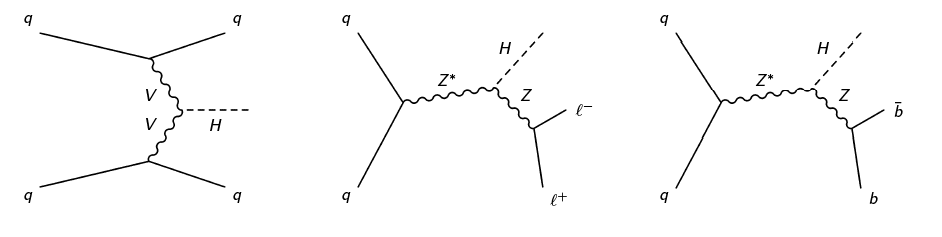
\includegraphics[width=\textwidth]{TalkPics/invcomb021213/feyndiags}
  %% \begin{fmfgraph*}(100,70)
  %%         \fmfleft{i1,i2}
  %%         \fmfright{o1,o2,o3}
  %%         \fmf{fermion}{i1,v1,o1}
  %%         \fmf{fermion}{i2,v2,o3}
  %%         \fmf{phantom,tension=4/5}{v1,v2}
  %%         \fmffreeze
  %%         \fmf{photon,label=$W,,Z$}{v1,v3}
  %%         \fmf{photon,label=$W,,Z$}{v2,v3}
  %%         \fmf{dashes}{v3,o2}
  %%         \fmflabel{$q$}{i1}
  %%         \fmflabel{$q$}{i2}
  %%         \fmflabel{$q$}{o1}
  %%         \fmflabel{$q$}{o3}
  %%         \fmflabel{$H$}{o2}
  %%       \end{fmfgraph*}
}
\date{}
\begin{document}
\begin{fmffile}{higgsexoupdatefeyndiags}

%TITLE PAGE
\section{Title}
\begin{frame}
  \titlepage
  
\end{frame}

\begin{frame}
  \frametitle{Overview}
  \begin{block}{}
    \scriptsize
    \begin{itemize}
    \item Preapproval conditions answered before Christmas
    \item Further study of single mu data suggested
    \item[-] Completed last week
    \item Unblinded results have been obtained and will be shown below
    \end{itemize}
  \end{block}
\end{frame}

\begin{frame}
  \frametitle{Unblinded yields}
  \begin{block}{}
    \centering
    \begin{tabular}{|l|c|}
      \hline
      Background       & $N_{est} \pm (stat) \pm (syst)$ \\
      \hline
      $Z\rightarrow\nu\nu$&$157.3 \pm 37.1 \pm 38.3$\\
      $W\rightarrow\mu\nu$&$101.8 \pm 6.1 \pm 11.9$\\
      $W\rightarrow e\nu$&$57.4 \pm 7.3 \pm 7.0$\\
      $W\rightarrow\tau\nu$&$98.0 \pm 13.2 \pm 25.4$\\
      top&$4.4 \pm 1.0 \pm 1.4$\\
      VV&$3.8 \pm 0.0 \pm 0.7$\\
      QCD multijet &$17\pm 0 \pm14$\\
      \hline
      Total Background &$439.7 \pm 40.5 \pm 55.8 $\\
      \hline
      Signal(VBF 125) &$273.4 \pm 0.0 \pm 31.2 $\\
      Signal(ggH 125) &$22.6 \pm 0.0 \pm 15.6 $\\
      \hline
      Observed & {\textcolor{red}{508}} \\
      \hline
    \end{tabular}
  \end{block}
\end{frame}

\begin{frame}
  \frametitle{Limits}
  \vspace{-.2cm}
  \begin{block}{}
    \scriptsize
    \begin{itemize}
    \item Prefit expected limit on B(H$\rightarrow$inv) 42\% for $m_{H}$=125 GeV from Asymptotic
    \item[-] 39\% with full toys, difference is due to a known feature of combines handling of pre-fit gmN when using Asymptotic
    \item Postfit observed (expected) limit on B(H$\rightarrow$inv) {\textcolor{red}{60}} (45)\% for $m_{H}$=125 GeV
    \item[-] This corresponds to a 1$\sigma$ upwards fluctuation
    \end{itemize}
  \end{block}
  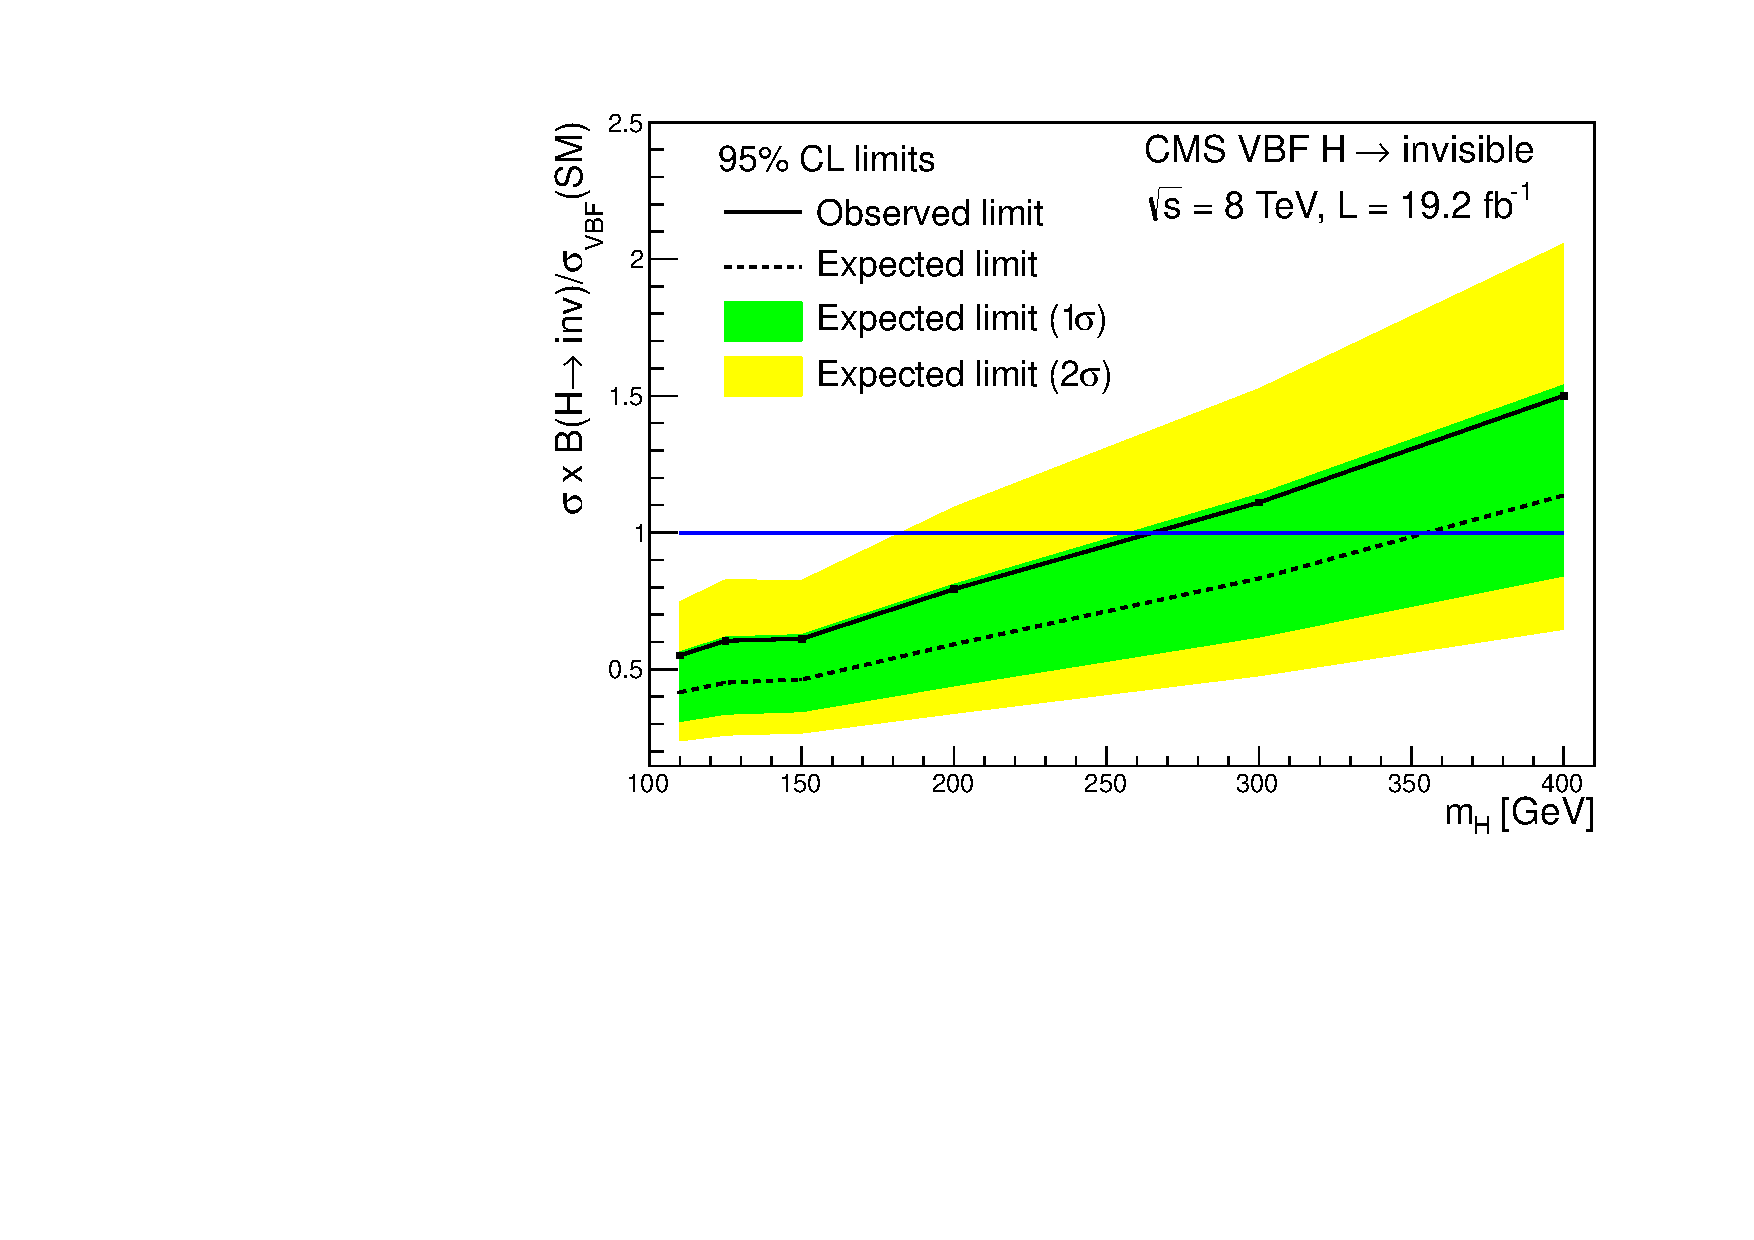
\includegraphics[width=.5\textwidth]{TalkPics/unblindedresult120114/vbflimit.pdf}
  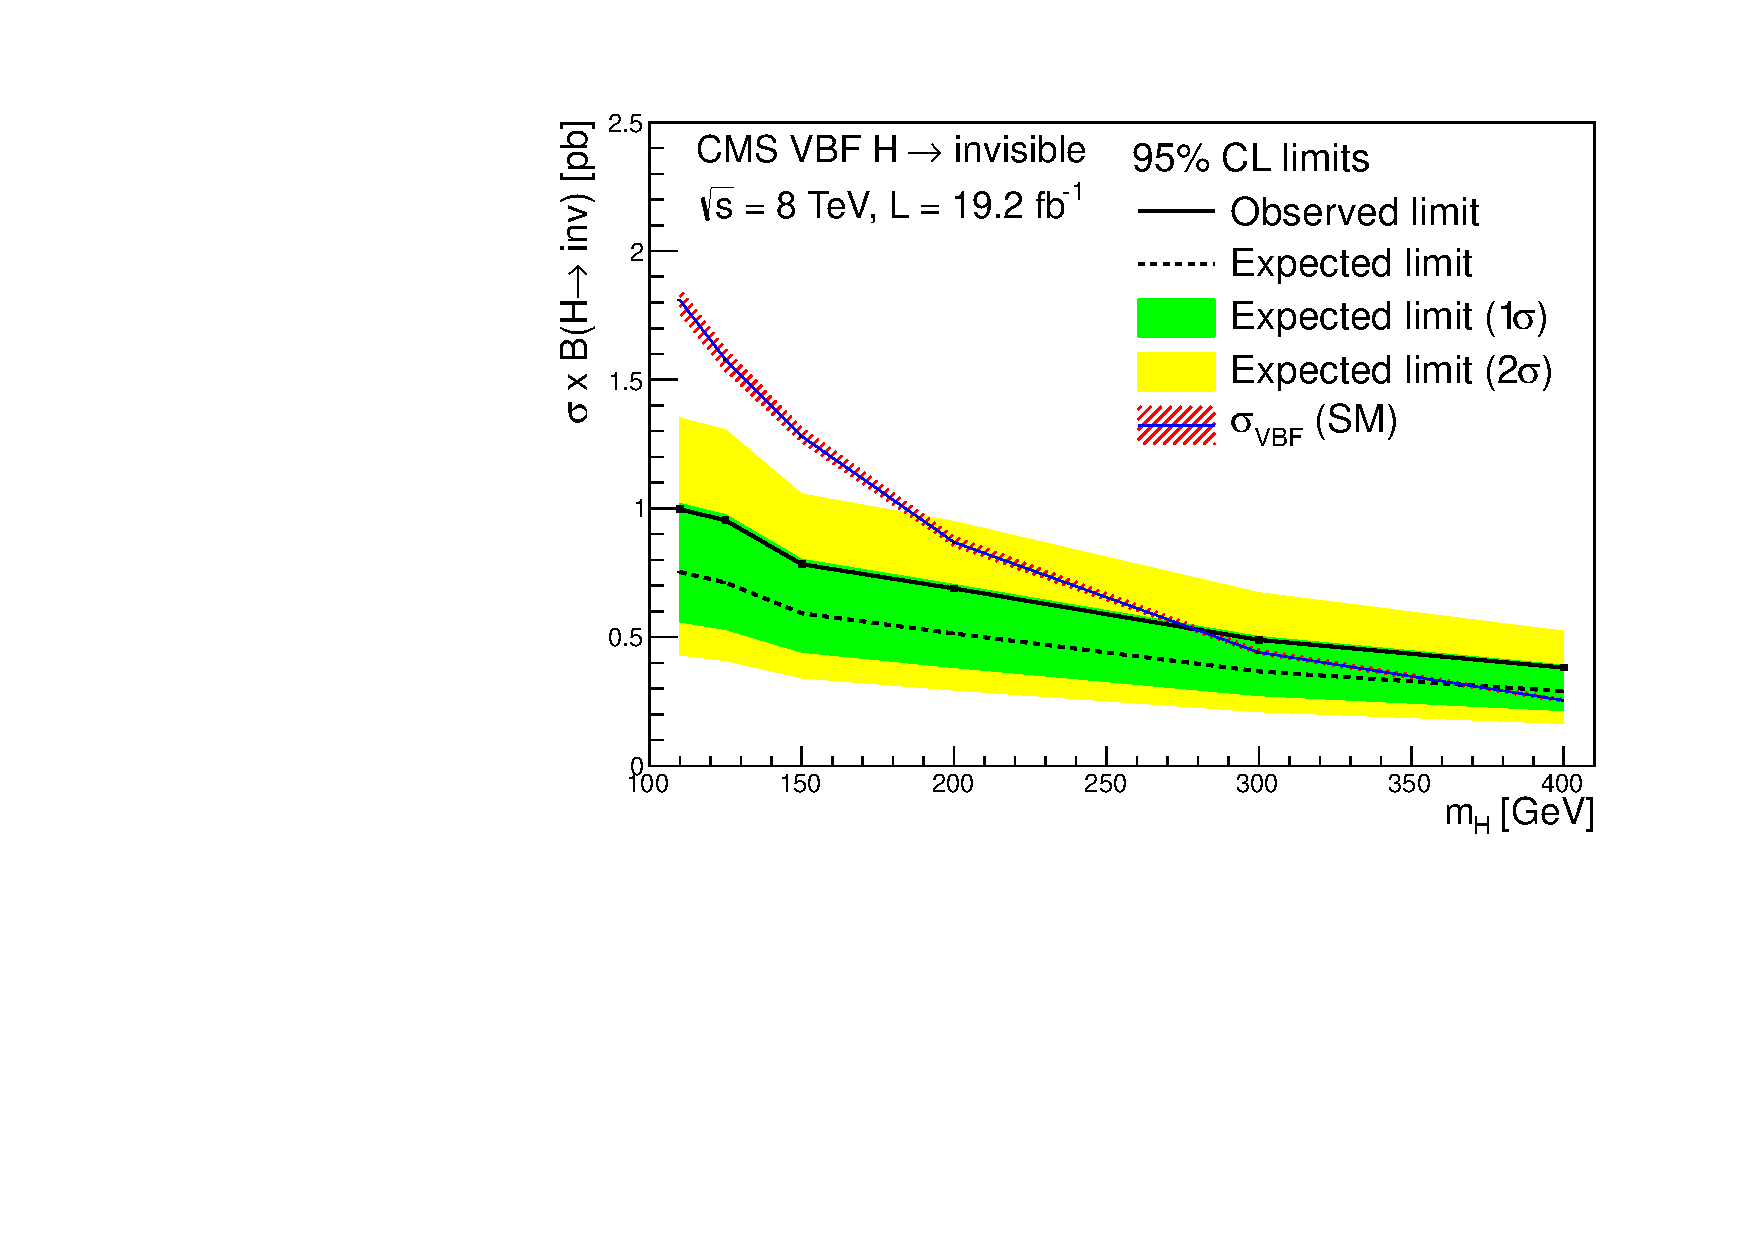
\includegraphics[width=.5\textwidth]{TalkPics/unblindedresult120114/vbfxslimit.pdf}
  \vspace{-.2cm}
  \begin{block}{}
    \scriptsize
    \begin{itemize}
    \item Single bin counting experiment so limit 100\% correlated across all mass points
    \end{itemize}
  \end{block}
\end{frame}

\begin{frame}
  \frametitle{Conclusion}
  \label{lastframe}
  \begin{block}{}
    \scriptsize
    \begin{itemize}
    \item Unblinded results shown
    \item We observe a 1$\sigma$ upwards fluctuation
    \item This gives us a postfit observed (expected) limit on B(H$\rightarrow$inv.) of {\textcolor{red}{60}} (45)\% for $m_{H}$=125 GeV
    \item[-] This limit includes a 20\% uncertainty on the $Z/\gamma^{*}\rightarrow\mu\mu$ to $Z\rightarrow\nu\nu$ extrapolation factor which is under investigation
    \item Documentation has been updated
    \end{itemize}
    
  \end{block}

\end{frame}

\begin{frame}
  \frametitle{Backup}
\end{frame}

\end{fmffile}
\end{document}
